%********** Chapter 2 **********
\chapter{Error Function}
\minitoc
In this chapter we are going to discuss several functions related to error function, namely, the error function itself, the complementary error function, and the inverse of the errof function.


\section{Error Function}
The error function is defined as the following integral
\[ \operatorname{erf}(x) = \frac{2}{\sqrt{\pi}} \int_0^x e^{-t^2}dt\]
where x belongs to $(-\infty, \infty)$. The scaler in front of the integral is to normalize the function between -1 and 1. Here are some basic facts:
\begin{enumerate}
\item the range is between -1 and 1.
\item $\operatorname{erf}(+\infty) = 1$ and $\operatorname{erf}(-\infty) = -1$.
\item $\operatorname{erf}(x)$ is strictly monotonely increasing.
\item $\operatorname{erf}(x)$ is an odd function.
\item the derivative is $\frac{2}{\sqrt{\pi}}e^{-x^2}$
\item the antiderivative is $x\operatorname{erf}(x) + \frac{1}{\sqrt{\pi}}e^{-x^2}$
\end{enumerate} 
The graph of the error function is below. 
\begin{figure*}[htp]
\begin{center}
{
%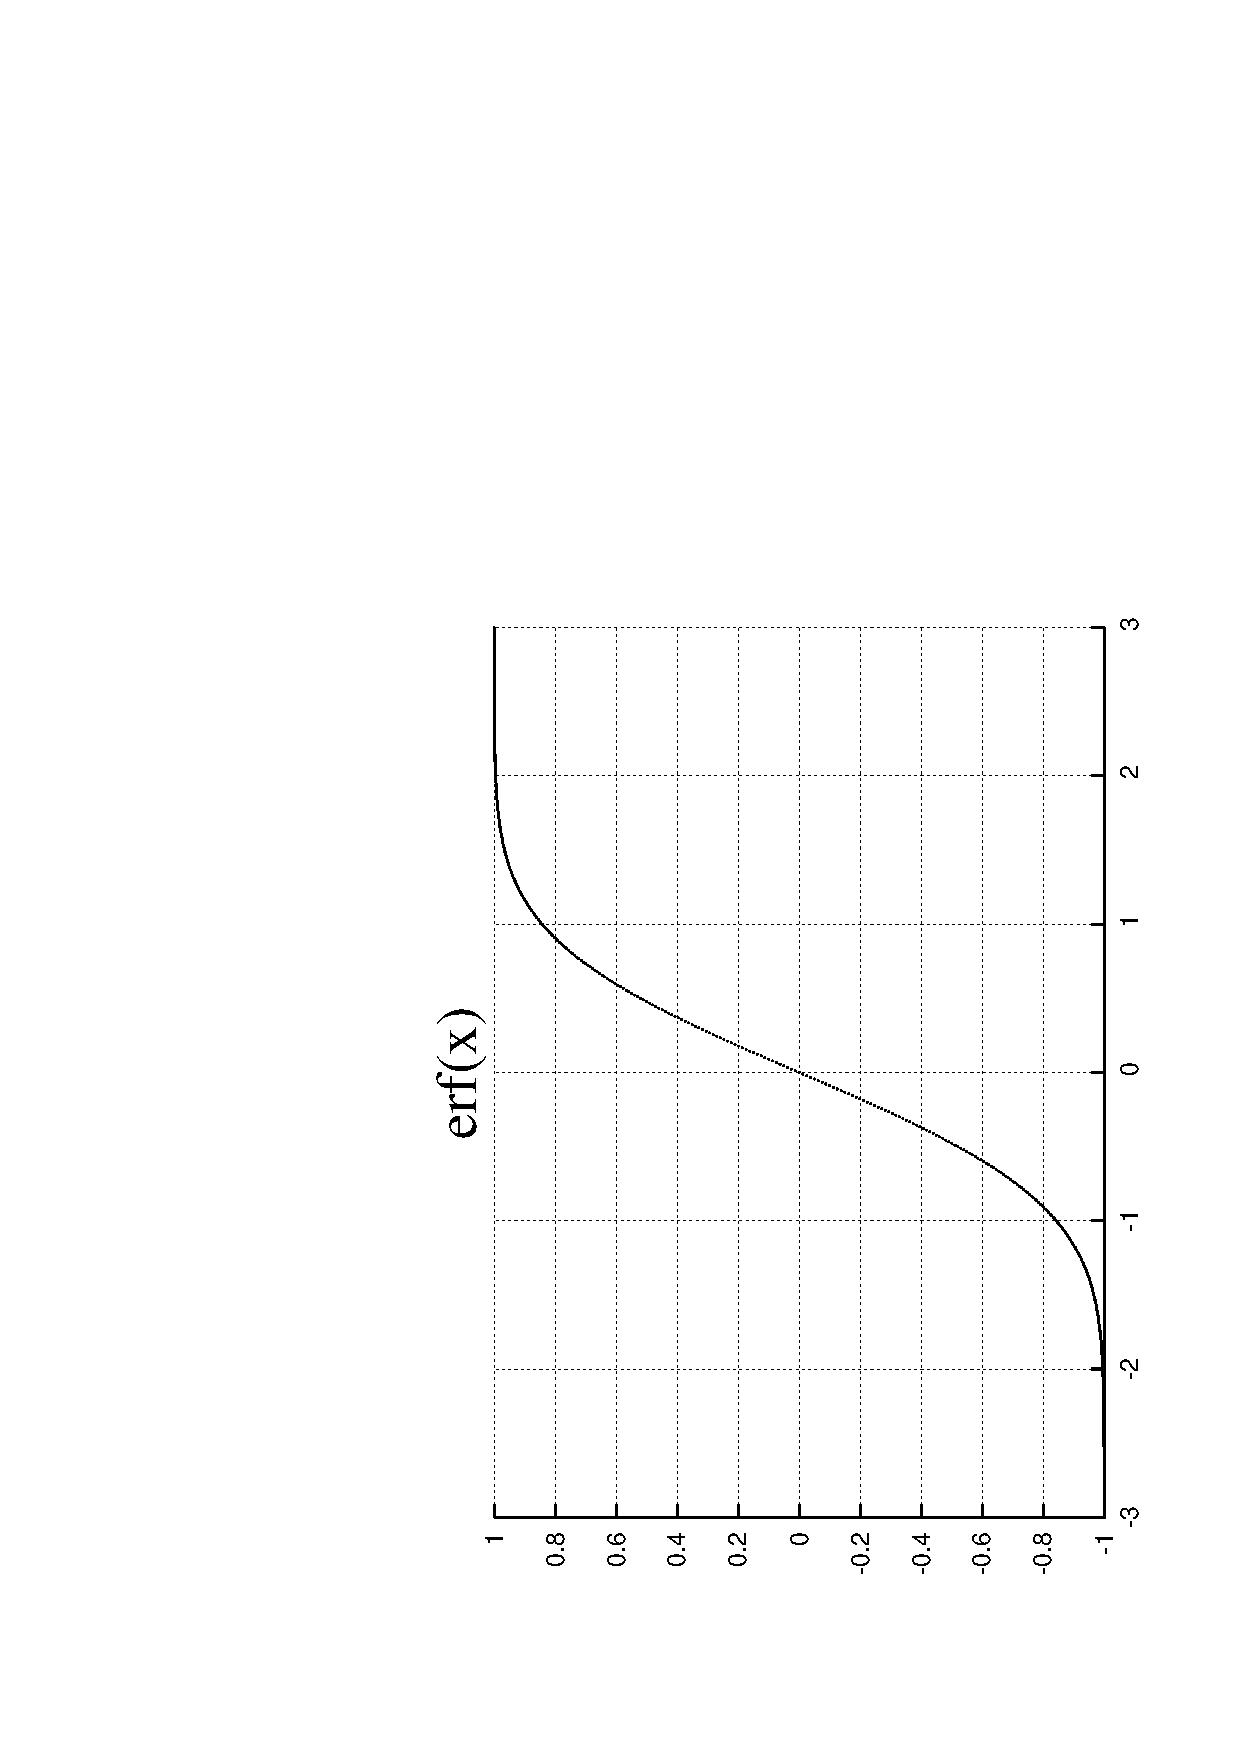
\includegraphics[bb=-90 0 400 250,width=1\textwidth] {chap2/erf}
\includegraphics[angle=-90,width=100mm]{chap2/erf.eps}
}
\end{center}
\caption{Error Function, from wiki}
\label{figure:errorfunction}
\end{figure*}

The implementation is a Java translation of c code from fdlibm53 written by Sun. There are a few ways to implement the error function, such as numerical integration, taylor expansion. But Sun's implementation is accurate and fast. The accuracy is 1ulp, the performance is ?ms per call on average.

\section{Complementary Error Function}
The complementary error function is defined as the following integral
\[ \operatorname{erfc}(x) = \frac{2}{\sqrt{\pi}} \int_x^{+\infty} e^{-t^2}dt\]
over the interval $(-\infty, \infty)$. $erfc(x)$ is the same integral as the error function, except the integral range now is over $(x, \infty)$ rather than $(0, x)$. It is easy to show 
\[ erf(x) + erfc(x) = 1\]
Here are more basic facts:
\begin{enumerate}
\item the range is between 0 and 2.
\item $erf(+\infty) = 0$ and $erf(-\infty) = 2$.
\item $erf(x)$ is strictly monotonely decreasing.
\end{enumerate}
The graph of the error function is below. 
\begin{figure*}[htp]
\begin{center}
{
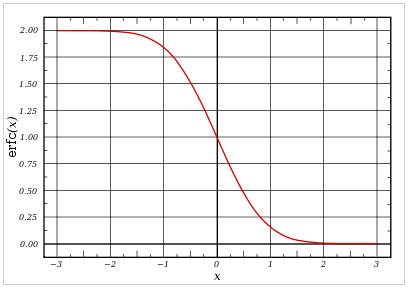
\includegraphics[bb=-90 0 400 250,width=1\textwidth] {chap2/errorcfunction.png}
}
\end{center}
\caption{Complementary Error Function, from wiki}
\label{figure:errorcfunction}
\end{figure*}

One way to implement $erfc(x)$ is to use $1 - erf(x)$. However, when x is large and $erf(x)$ is near 1, this suffers from cancellation error. One way to fix this is to use BigDecimal when x is large.

Fortunately, Sun's fdlibm53 has an implmentation for the complementary error function too. The accuracy is 1ulp, the performance is ?ms. 


\section{Error Function Inverse}
Since the error function is strictly increasing on the entire real axis, the inverse function exists in $(-1, 1)$. The implementation is a translation of c code from cephes. performance? 



%********** End of chapter **********
